\newpage
\section{Theoretische Grundlagen}
\textcolor{red}{Quellen überall ergänzen} \\
Im folgenden Teil der Ausarbeitung werden die theoretischen Grundlagen zum Verständnis der Ausarbeitung erläutert.
Zunächst wird der \ac{OSMI} als Hautpaugenmerk erklärt. Es folgen der Oberbegriff Deep Learning und die dazugehörige Methode der Bildklassifizierung.
Darauf folgt das \ac{NLP} mit der \ac{NER}.

\subsection{Online Sensory Marketing Index}

Der Fokus in dieser Ausarbeitung liegt auf dem \acl{OSMI}. Es handelt sich dabei um ein Bewertungsinstrument, welches im Jahr 2018 entwickelt wurde.\textcolor{red}{Zitat}
Ziel des \ac{OSMI} ist es, dass E-Commerce Webseiten im Hinblick auf deren sensorische Gestaltung bewertet werden und dementsprechend Verbesserungspotentiale aufgezeigt werden.
Unter einer sensorischen Gestaltung werden Parameter gefasst, die sich nach den Sinnen eines Menschen richten. Diese sind die Haptik, die Olfaktorik, die Akustik, die Gustatorik und die Visualität.\textcolor{red}{Zitat}
Die Bewertung im \ac{OSMI} wird anhand verschiedener Indikatoren der einzelnen Sinne vorgenommen. Nachfolgend sind beispielhafte Indikatoren der einzelnen Sinne aufgeführt, die im \ac{OSMI} Berücksichtigung finden:

\begin{itemize}
    \item Haptik: 3D-Bilder, Video, Endowment-Effekt, …
    \item Olfaktorik: Mentale Simulation von Düfte, Schlüsselbegriffe für Düfte
    \item Auditive: Töne/Musik, Sprecher/Stimme, Schlüsselbegriffe für Akustik, …
    \item Gustatorische: Mental Simulation des Schmeckens, Verwendung von
    Farbschemata, Produktoptio \& Oberflächen, …
    \item Visuelle: Farbgebung, dynamische Bilder, Oberfläche, …
\end{itemize}

Die Evaluation der einzelnen Indikatoren wird in Form einer Tabelle dargestellt. Ein Beispiel ist am Ende dieses Kapitels aufgeführt \textcolor{red}{ref label der tabelle}.
Für eine Webseite wird jeder Indikator der fünf Sinne einzeln bewertet und auf Basis dessen letztendlich für jeden der fünf Parameter ein Wert zwischen 0 und 1 ermittelt.
Eine Gewichtung zwischen den einzelnen Indikatoren wird dabei nicht vorgenommen. \\
Im letzten Schritt zur Ermittlung des \ac{OSMI} wird über die Parameter der fünf Sinne das arithmetische Mittel berechnet.
Dieser Wert liegt ebenfalls zwischen 0 und 1 und bildet den \ac{OSMI} einer Webseite. Dabei gilt, dass die Webseite erfolgreicher die Sensorik anspricht, wenn der OSMI-Index näher an einer 1 liegt.
Liegt der Wert näher an einer 0 werden schlussfolgernd wichtige Elemente zur Ansprache der Sensorik nicht genutzt. \\
Die nachfolgende Tabelle zeigt ein Beispiel aus der Masterarbeit von K.Hamacher zum \ac{OSMI} der Webseite \textit{www.mymuesli.de}.

\textcolor{red}{mymuesli Beispiel ergänzen? Hier noch was zu schreiben?}


\subsection{Deep Learning}

Die Image Classification ist ein Anwendungsfall für die Technik des Deep Learning.
Als Teilgebiet des Machine Learning bedient sich das Deep Learning mehrschichtiger neuronaler Netze, welche auf Basis großer Datenmengen bereits Erlerntes mit neuen Inhalten verknüpft und somit wiederum erneut lernt.\textcolor{red}{Zitat}
Deep Learning macht es möglich, dass eine Maschine selbstständig die Gewichtungen seines verwendeten Modells verbessert.
Anwendungsbereiche für Deep Learning können beispielsweise die Gesichts-, Objekt- oder Spracherkennung sein. \textcolor{red}{Zitat je Anwendungsfall} Die Anwendung der Objekterkennung wird nachfolgend beschrieben.

\subsubsection{Image Classification}
Bei der Image Classification handelt es sich um eine Technik, bei der ein Objekt auf einem Bild einer bestimmten Klasse zuordnet wird. Als Ziel kann die genaue Identifizierung der Bildmerkmale verstanden werden.
Es gibt verschiedene Methoden, die zur Image Classification eingesetzt werden können wie die Supervised Classification, die Unsupervised Classification oder auch die \acp{CNN}.\textcolor{red}{Zitat}
Letzteres wird am häufigsten für den Anwendungsfall herangezogen.\textcolor{red}{Zitat}

\subsubsection{Convolutional Neural Network}
Das \ac{CNN} ist eine besondere Form eines künstlichen neuronalen Netzes. Es zeichnet sich durch mehrere Schichten wie den Convolutional- Layer, den Pooling Layer und den Fully-Connected Layer aus.
Die Architektur ist in der Abbildung ref{fig:CNN} dargestellt.
\\

\begin{figure}[H]
    \caption{Aufbau des Convolutional Neural Networks}\label{fig:CNN}
    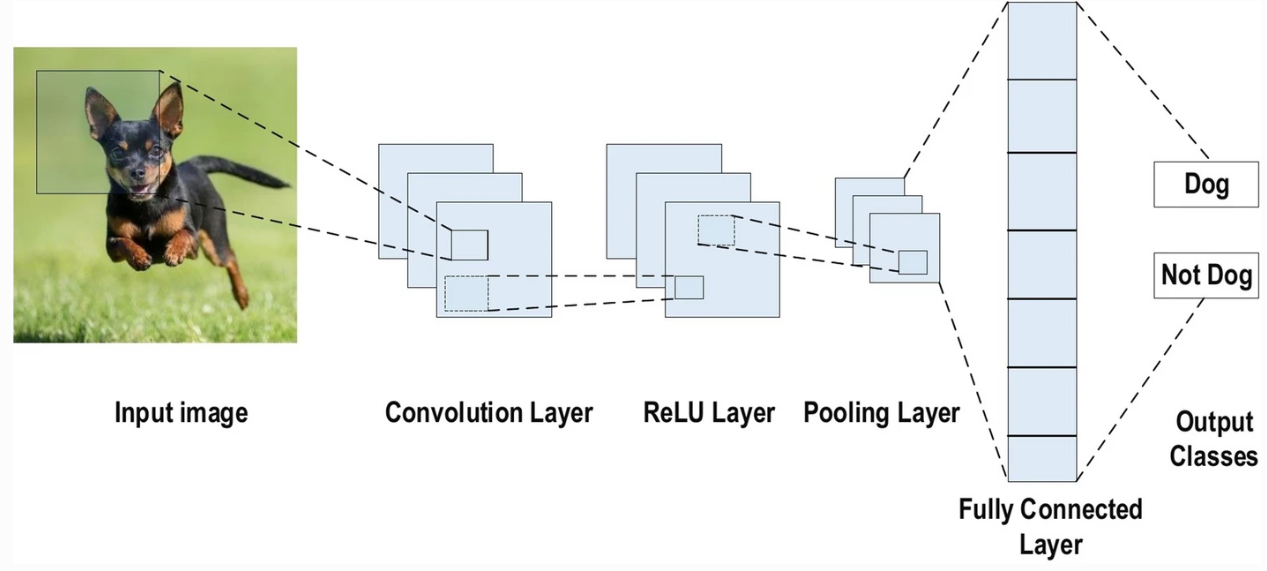
\includegraphics[width=0.9\textwidth]{CNN}
    \textit{Quelle:~\cite[][\pagef 14]{alzubaidiReviewDeepLearning2021}}
\end{figure}

In den Schichten der Convolution werden die Eingabebilder analysiert und Merkmale (zum Beispiel Linien oder Kanten) der Bilder erkannt und extrahiert.
Die Verarbeitung dieser Merkmale erfolgt in Matrizen, die Feature Maps genannt werden. \\
Die Feature Maps als Ausgabe der Convolutional Layer werden darauf in den Pooling Layer eingegeben.
Die Größe der Bilder wird in dieser Schicht reduziert und durch Methoden wie dem Max-Pooling nur die wesentlichen Merkmale weitergegeben.
Alle anderen Informationen sind für die Verarbeitung überflüssig und werden verworfen. Ergebnis dieser Schicht ist die gleiche Anzahl an Feature Maps, allerdings in komprimierter Form. \\
Der Fully-Connected Layer bildet den Abschluss der \ac{CNN}-Architektur. Jeder Knoten in der Ausgabeschicht ist hier direkt mit einem Knoten der vorgelagerten Schicht verbunden.
Mithilfe einer Linearkombination und einer Aktivierungsfunktion wird schlussendlich das Bild klassifiziert. Die Zuordnung zu einer Klasse erfolgt dabei auf Basis einer Wahrscheinlichkeit.

\subsection{Natural Language Processing}
Die \acl{NER} ist eine Technik, welche dem Oberbegriff des \acl{NLP} zugeordnet wird. Das \ac{NLP} beschäftigt sich mit der Verarbeitung und dem Verständnis der menschlichen Sprache durch einen Computer.\textcolor{red}{Zitat}
Ziel dieser Techniken ist es eine direkte Kommunikation zwischen dem Menschen und dem Computer mithilfe der Sprache herzustellen. Die Fachgebiete der Computerlinguistik, Informatik, Kognitionswissenschaft und künstlicher Intelligenz werden hier vereint.
Anwendungsfälle können beispielsweise die Extraktion der Bedeutung von Sätzen oder Satzteilen oder auch die Erkennung von Satzzusammenhängen sein. Neben Techniken wie der Sentiment-Analyse und der Spracherkennung gehört auch die \acl{NER} zu den Funktionen des \ac{NLP}.

\subsubsection{Named Entity Recognition}
Die \acl{NER} hat zur Aufgabe automatisiert Entitäten in einem Textdokument zu finden und zu klassifizieren.\textcolor{red}{Zitat} Letzteres geschieht anhand zuvor definierter Kategorien.
Eine Entität muss dabei nicht unbedingt nur aus einem einzelnen Wort bestehen, sondern kann auch eine Reihe von Wörtern umfassen, solange sie sich auf dieselbe Sache beziehen.

\subsubsection{Vorgehen bei der NER}
In der \ac{NER}-Technik werden zwei Schritte durchgeführt, um zu Ergebnissen zu gelangen:

\begin{enumerate}
    \item Erkennen einer Entität
    \item Kategorisierung der Entität
\end{enumerate}


Im ersten Schritt wird geprüft, ob eine Wortfolge eine Entität bildet. Die Anfangs- und Endgrenzen der Entitäten werden hierbei festgelegt. Der zweite Schritt hat zum Ziel die zuvor definierte Entität in eine der zuvor definierten Klassen einzuordnen.
Häufig verwendete Klassen sind beispielsweise Orte, Namen oder Organisationen, welche unter die generischen Kategorien fallen.\textcolor{red}{Zitat} Des Weiteren gibt es domänenspezifische Kategorien wie zum Beispiel Proteine, Enzyme oder Gene.
\\
Zur Durchführung der beiden Schritte gibt es verschiedene Ansätze, die angewendet werden können. Ausgehend von den annotierten Datensätzen, die beispielsweise aufgrund von manuell erstellten Regeln oder auf Basis von Kontextähnlichkeiten generiert werden, werden Modelle mithilfe von Machine Learning entwickelt.
Für zuvor ungesehene Daten ermitteln die Modelle Vorhersagemodelle zur Erkennung und Kategorisierung der Entitäten. Eine weitere Möglichkeit ist der Einsatz von Deep Learning zur \ac{NER}. In diesem Ansatz können auch nicht-lineare Zusammenhänge erkannt und gelernt werden.\textcolor{red}{Zitat}
\\
Ein Beispiel für ein Textdokument, in dem die \ac{NER} Technik angewendet wurde, ist in Abbildung \textcolor{red}{ref xy} dargestellt.\\


\begin{figure}[H]
    \caption{Beispiel der \ac{NER} Technik}
    \label{fig:NLP}
    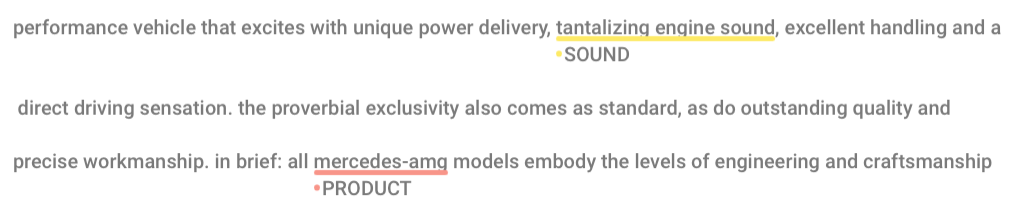
\includegraphics[width=1\textwidth]{NLP.png}
    \textit{Quelle: Eigene Darstellung}
\end{figure}

Die \ac{NER}-Technik kann in unterschiedlichen Bereichen angewendet werden. Zum Beispiel können durch die Anwendung die Antwortzeiten im Kundendienst verringert werden, indem die Anfragen zuvor kategorisiert oder direkt dem zuständigen Mitarbeiter zugeordnet werden.\textcolor{red}{Zitat}
\\
Um die Qualität der \ac{NER}-Technik zu bewerten, werden die Kennzahlen Precision, Recall und der F-Score hinzugezogen.
Zur Ermittlung dieser muss zunächst die Anzahl der Entitäten mit verschiedenen Ausprägungen ermittelt werden (\ac{FP}, \ac{FN}, \ac{TP}).

\begin{itemize}
    \item \ac{FP}: Eine Entität wurde erkannt, obwohl sie keine darstellt
    \item \ac{FN}: Eine Entität wurde nicht erkannt, obwohl sie eine darstellt
    \item \ac{TP}: Eine Entität wurde richtig erkannt
\end{itemize}

Die Precision zeigt das Verhältnis zwischen richtig erkannten Entitäten und der Gesamtheit der identifizierten Entitäten an. Die Formel lautet wir folgt:
\begin{align}
    Precision {=} \frac{\ac{TP}}{(\ac{TP}+{\ac{FP}})}
\end{align}
Der Recall stellt den Anteil der richtig erkannten Entitäten an der Gesamtheit aller möglichen Entitäten dar.
\begin{flalign}
    Recall{} {=} {}\frac{\ac{TP}}{(\ac{TP}+{\ac{FN}})}
\end{flalign}
Der F-Score ist die Kennzahl, der die Precision und den Recall zu einem harmonischen Mittel vereint:
\begin{flalign}
    F-Score{} {=} {}2 \cdot \frac{Precision \cdot Recall}{Precision + Recall}
\end{flalign}
